\documentclass{article}
\usepackage[T1]{fontenc}

\usepackage{graphicx}
\usepackage{listings}
\begin{document}

\title{FOSS Lab Report}
\author{Gokul K\\[2\baselineskip]
Roll Number: 21\\[2\baselineskip]}
\date{25 January 2020}

\maketitle

\setcounter{section}{5}
\section{Shell Programming III}
\subsection{Aim}
Write a shell script to implement a menu driven calculator with following functions\newline
  1) Addition\newline
  2) Subtraction\newline
  3) Multiplication\newline
  4) Division\newline
  5) Modulus\newline
\subsection{Source Code}
\begin{verbatim}
#! /bin/bash
clear
i="y"
echo "Enter First number"
read num1
echo "Enter second number"
read num2
while [ $i = "y" ]
do
	echo "1 - Sum"
	echo "2 - Difference"
	echo "3 - Product"
	echo "4 - Quotient"
	echo "5 - Remainder"
	read c

	case $c in
		1) sum=`expr $num1 + $num2`
		echo "Sum = "$sum
		;;

		2) sum=`expr $num1 - $num2`
		echo "Difference = "$sum
		;;

		3) sum=`expr $num1 \* $num2`
		echo "Product = "$sum
		;;

		4) sum=`expr $num1 / $num2`
		echo "Quotient = "$sum
		;;

		5) sum=`expr $num1 % $num2`
		echo "Remainder = "$sum
		;;
	esac

	echo "Continue (y/n)?"
	read i
	if [ $i != "y" ]
	then
		exit
	fi
done
\end{verbatim}

\subsection{Output}
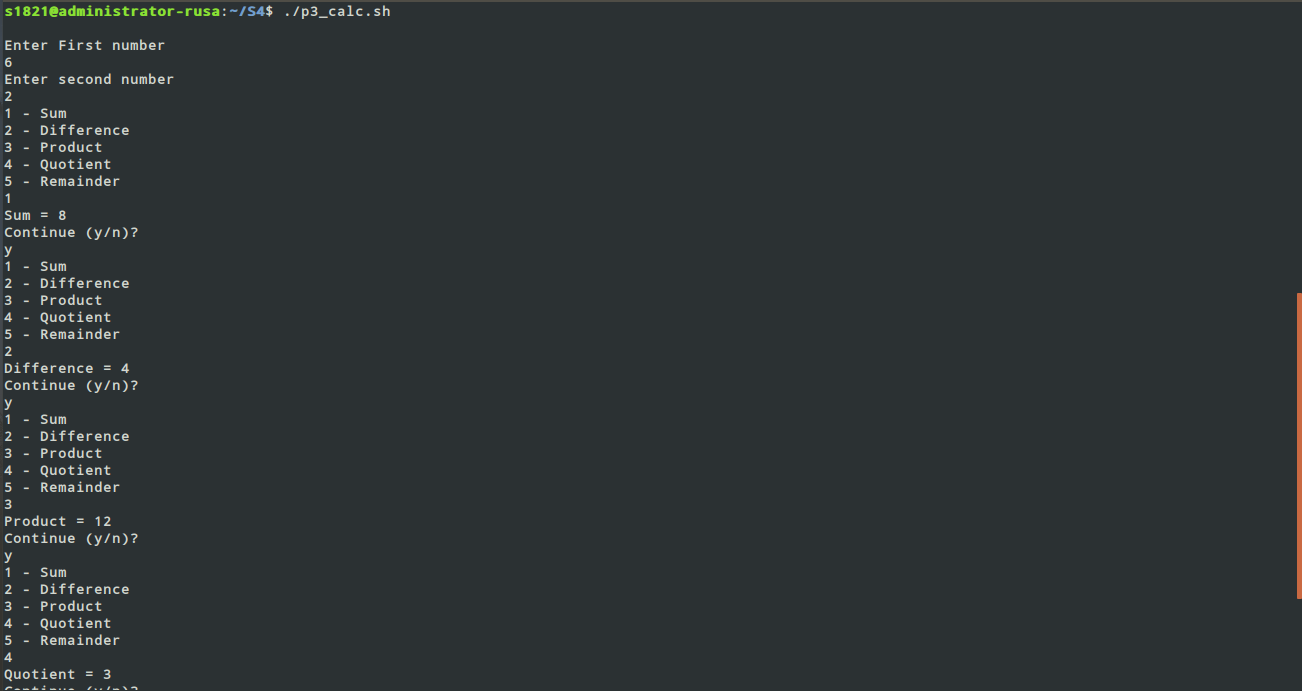
\includegraphics[width=0.9\textwidth]{img/p6/ss1.png}\newline
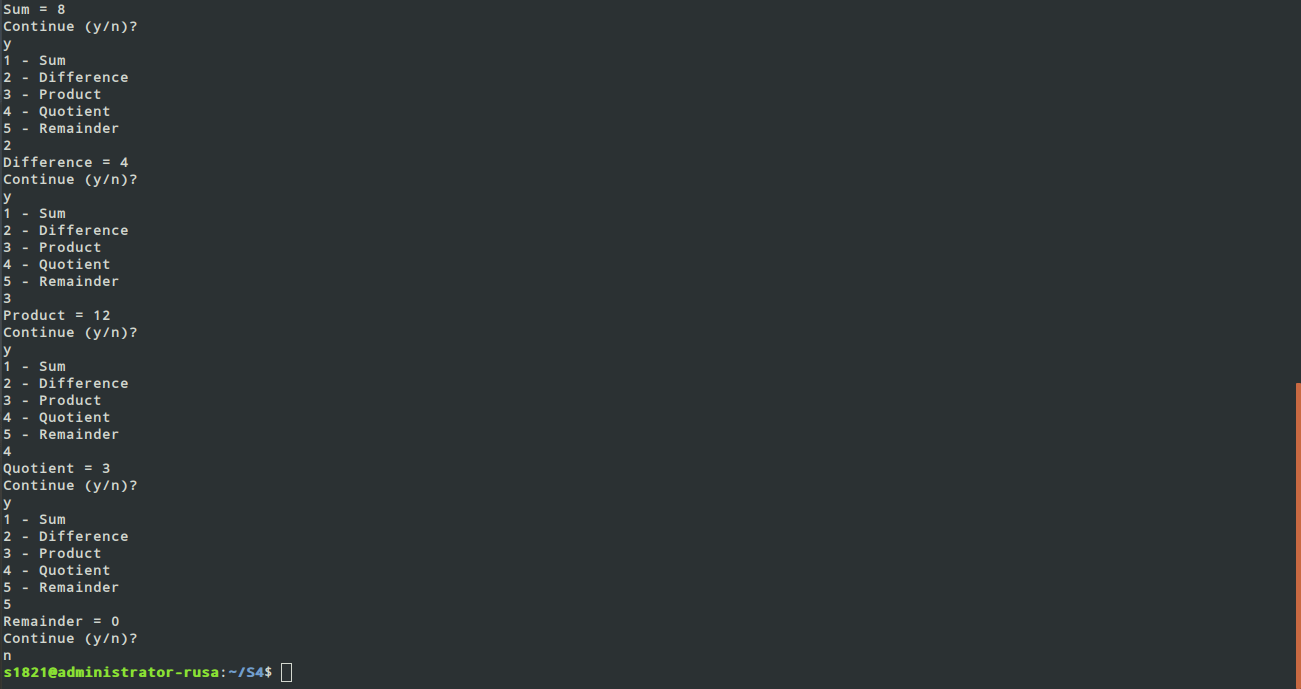
\includegraphics[width=0.9\textwidth]{img/p6/ss2.png}\newline

\subsection{Result}
The above program is run on the server shell. Sample inputs were given and the outputs were recorded.
\end{document}